\documentclass[a4paper,twoside]{article}
\usepackage{epsfig}
\usepackage{subcaption}
\usepackage{calc}
\usepackage{amssymb}
\usepackage{amstext}
\usepackage{amsmath}
\usepackage{amsthm}
\usepackage{multicol}
\usepackage{pslatex}
\usepackage[T1]{fontenc}
\usepackage[utf8]{inputenc}
\usepackage{apalike}
\usepackage{algorithm2e}
\usepackage[bottom]{footmisc}
\usepackage{array}
\usepackage{fvextra}
\usepackage{url}
\usepackage[hidelinks,pdfauthor={},pdfcreator={},pdfproducer={},pdftitle={Finite-Packet Limits and Public Recognition in LLM-Based Encrypted Text Transport},pdfsubject={},pdfkeywords={}]{hyperref}
\usepackage{SCITEPRESS}
\pdfinfoomitdate=1
\pdftrailerid{}
\newcommand{\aidraft}{\footnote{Drafting assistance: \cite{openai2026codex}. See the AI-use disclosure.}}

\begin{document}
\title{Finite-Packet Limits and Public Recognition in LLM-Based Encrypted Text Transport}
\author{}
\keywords{Linguistic Steganography, Public-Key Encryption, Arithmetic Coding, Text Transport, Traffic Recognition.}
\abstract{Encrypting a payload before embedding it in language-model text separates content confidentiality from recognition of communication. We study this separation under an actual UTF-8 transport contract using one frozen quantized model, a common admissible token support, and public rank and arithmetic comparators. An independent reconstruction of retained arithmetic failures identifies low-information trajectories rather than an incorrect inverse. Extending one carrier ceiling preserves earlier trajectories but leaves all four fresh 128-byte arithmetic attempts incomplete. A six-context prospective study then pairs probability-weighted controls that share a sampling trajectory but use different stopping rules. Four of six encrypted messages recover exactly, while three of six controls stopped at packet completion are delivered. Matching the stopping rule removes the completion-boundary distinction on those controls, but canonical packet replay rejects all three. A separately selected historical prefix passes the public format, illustrating that acceptance is not authentication. These small, separate cohorts support a bounded empirical account of capacity, stopping and finite-packet conformance. They do not establish concealment against human traffic, population detector performance, or a new cryptographic construction.}
\onecolumn\maketitle\normalsize\setcounter{footnote}{0}\vfill

\section{INTRODUCTION}
\label{sec:intro}
\noindent Encryption can hide what a message says while leaving the use of encryption obvious. Linguistic steganography attempts to hide communication inside text. A language model offers a way to generate that text while selecting tokens that carry information. A \emph{token} is a model vocabulary item, which may be a word, part of a word, punctuation, or a byte fragment. The resulting text is the \emph{carrier}. The practical question is not only whether tokens encode bits. It is whether a complete message survives conversion to text, delivers its protected payload, and differs from an explicitly defined source of ordinary-looking text.\aidraft

These questions become distinct when the embedding algorithm, model and context are public. An observer can repeat the public extraction process and recover candidate encrypted bytes without possessing the recipient's private key. That ability need not reveal the plaintext, and it does not universally imply detectable communication. It becomes useful for recognition when the extracted bytes or the message boundary satisfy a public constraint that the comparison distribution rarely satisfies. Classical public-key steganography already makes such distribution and cryptographic assumptions explicit \cite{vonahn2004public}.

Finite messages create constraints that a token-level description can miss. A rank mapper can consume a fixed number of bits at each step while choosing improbable tokens. Arithmetic coding instead gives more probable tokens wider intervals, but a nearly deterministic continuation can consume many tokens while resolving almost no packet bits. Even after sufficient bits become recoverable, a particular finite-packet encoder may accept only one of several token paths consistent with that bit prefix. A \emph{stopping rule} specifies when generation ends. Different stopping rules can distinguish two sources that use exactly the same next-token sampling distribution.

We investigate these issues in public encrypted-text transport. Established Hybrid Public Key Encryption (HPKE) protects a small binary payload. Public codecs turn the resulting ciphertext envelope into text. The receiver begins with the transmitted UTF-8 byte string and its private key. Public diagnostics begin with the same text and agreed public parameters, without the key. We compare rank mapping with one adapted arithmetic method while holding the model and text-consistency filter fixed. We retain capacity failures and distinguish delivered-message recognition from all-attempt recovery.

The contribution is a bounded empirical decomposition, rather than a new encryption primitive or entropy coder. First, we connect exact text recovery to a documented serialization contract and retain failures of an audited rank-transcoding baseline. Second, independent arithmetic reconstruction and a single ceiling extension distinguish insufficient information accumulation from an inverse error. Third, paired controls isolate public first-completion stopping from deterministic finite-packet replay. The last distinction is tested prospectively and illustrated by a separate retrospective counterexample to interpreting format acceptance as proof of encryption.

The scope is small. In the final study, four of six arithmetic transmissions recover exactly and three of six stopped controls deliver. All three controls meet the completion boundary but fail canonical replay. These observations separate rejection mechanisms. They do not resolve a general recognition tradeoff.

\section{BACKGROUND AND RELATED WORK}
\label{sec:related}
\subsection{Public Extraction and Confidentiality}
\noindent A ciphertext envelope is the complete public object needed for decryption, including the key encapsulation and authenticated ciphertext. Its representation need not be uniformly random. A recognizer can exploit a representation constraint without learning the encrypted message. Conversely, public extraction can be compatible with secure steganography under appropriate channel assumptions. Von Ahn and Hopper's public-key constructions use a public extraction function and encryption with ciphertexts indistinguishable from random bits, together with conditions on the cover channel \cite{vonahn2004public}. We do not transfer their security theorem to a general HPKE serialization or to our model-generated channel.\aidraft

HPKE supplies encryption, not concealment \cite{rfc9180}. Base mode does not authenticate senders. A stranger can encrypt a fresh valid message to the public key without forging a tag. Our private receiver authenticates before returning payload bytes; the public observer never authenticates. No new security reduction for the combined transport is supplied.

\subsection{Rank and Probability Mapping}
\noindent Calgacus records source-token conditional ranks and selects the corresponding ranks under a different context \cite{norelli2026calgacus}. Its paper discusses difficult high-entropy inputs and distinguishes rank preservation from probability preservation. Our audited baseline applies that idea to canonical Base64 ciphertext using a different local model build, explicit tie ordering, cache handling and strict text serialization. It is an adaptation, not an unmodified replication. The bounded rank-16 profiles studied here are also separate methods. In particular, their public length header is our framing choice, not a property attributed to original Calgacus.

Ziegler et al. reverse arithmetic coding to map input bits into language-model output, with probability-dependent intervals and finite-message termination \cite{ziegler2019neural}. Their analysis also distinguishes a model distribution from natural language. Our arithmetic comparator retains that established mapping idea but uses a restricted, text-consistent alphabet and one explicit midpoint extension for finite packets. It is independently implemented after source inspection. No code from the inspected, unlicensed upstream tree is copied. These changes mean that our failures and format checks do not evaluate every arithmetic steganographic construction.

Meteor identifies variable entropy as a practical obstacle and explains why straightforward encrypted randomness need not preserve a realistic sampling distribution \cite{kaptchuk2021meteor}. Its construction uses synchronized secret pseudorandom state. We do not replace that secret with a public seed while retaining its security claims. Meteor is an analytical comparison, not an experimental baseline. Our question concerns bounded encrypted packets and public checks under one common admissible support.

\subsection{The Text Boundary}
\noindent Token decoding is not always inverted by retokenizing the rendered text. A receiver given only text may reconstruct different token IDs even when the sender's internal token-level inverse is correct. Yan and Murawaki explicitly address this problem with stepwise verification of the entire proposed prefix at both endpoints \cite{yan2025tokenization}. Our candidate rule follows that principle. Strict UTF-8, a bounded scan and a fixed alphabet size are engineering policies, not claimed inventions. The present experiments ask what happens after those policies are combined with finite encrypted packets and explicit cover-generation rules.

\section{TRANSPORT AND OBSERVER CONTRACT}
\label{sec:contract}
\subsection{Public and Private Inputs}
\noindent Figure~\ref{fig:protocol} separates public extraction from private recovery. Public information includes the recipient public key, exact cover context, model and tokenizer identities, numerical settings, token ordering, codec and framing policy. Where used, the payload-size class is a pre-agreed channel setting. The recipient private key and fresh encryption randomness are secret in the intended deployment. Experimental keys are harmless test fixtures, not operational secrets. Authentic distribution of the recipient public key is an external assumption. No secret prompt contributes to confidentiality.\aidraft

The transmitted object is a bounded UTF-8 byte string with an externally supplied message boundary. The receiver is given those bytes, public configuration and its private key. It receives no sender token IDs, rank lists, original envelope, expected payload hash or cached model state. Receiver traces are evaluator outputs. Independent receiver processes start from saved text, and the evaluator compares recovered hashes afterward. Repeating reception is a process-isolation check, not another independent transmission or a test that an application replay cache should accept duplicates.

\begin{figure*}[t]
\centering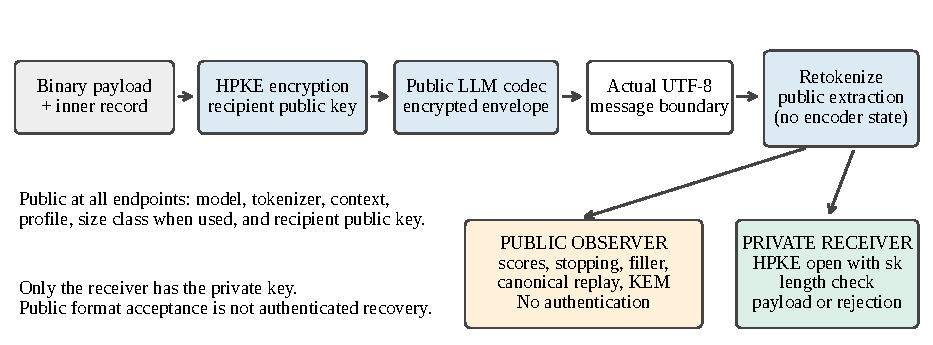
\includegraphics[width=\textwidth]{figures/figure1_protocol.pdf}
\caption{The actual-text contract. Both public checks and private recovery reconstruct from received UTF-8 and public configuration. The observer can recover candidate encrypted bytes and test their format; only the receiver opens HPKE with a private key. No diagnostic sender state crosses the text boundary. This is a scripted schematic, not a measurement; tool assistance is disclosed \cite{openai2026codex}.}
\label{fig:protocol}
\end{figure*}

\subsection{Encrypted Record and Binding}
\noindent The implementation uses pyhpke 0.6.5 and cryptography 46.0.7. The suite is Base-mode DHKEM(X25519, HKDF-SHA256), HKDF-SHA256 and ChaCha20-Poly1305. The authenticated inner record contains a fresh 16-byte random message identifier, a four-byte unsigned big-endian payload length and the payload. There is no padding. The public envelope concatenates the 32-byte encapsulation with ciphertext and its 16-byte tag. An $n$-byte payload therefore needs $n+68$ envelope bytes. The two experimental classes are 32 and 128 useful bytes, corresponding to 100 and 196 envelope bytes.

The complete profile and selected context are encoded in sorted, length-framed canonical JSON. Domain-separated HPKE information binds those bytes; associated data bind their SHA-256 digest. Changed contexts or ceilings receive new profiles and fresh encryption. Old-envelope diagnostics open ciphertext only under its original authenticated binding. Transport bounds are checked before allocation, and private recovery validates the authenticated inner length before returning payload bytes.

\subsection{A Common Canonical Alphabet}
\noindent Let $T$ tokenize text bytes and $D$ detokenize token IDs. At each step, we sort the model's float32 logits in descending order, breaking exact ties by ascending token ID. We scan at most the first 128 IDs. Special or control tokens and tokens with empty emitted bytes are excluded. A candidate $v$ after carrier prefix $x$ is admitted only if $D(xv)$ is strict UTF-8 and
\begin{equation}
T(D(xv))=xv.
\label{eq:canonical}
\end{equation}
The first 16 admitted candidates form the ordered support. Fewer than 16 cause an explicit admissibility failure. We do not enlarge the scan or replace an output token after failure. Detokenization tests the entire carrier prefix, not concatenated singleton token strings. The public context initializes the model but is not silently prepended to the transmitted text.

Every admitted prefix has the intended canonical tokenization. Identical logits, ordering and tokenizer behavior let sender and receiver reconstruct the same candidates. This conditional correctness invariant neither guarantees portability across backend builds nor establishes concealment. The constrained distribution differs from unrestricted model sampling and human text.

\begin{table*}[t]
\caption{Evaluated transport profiles. All encrypted rows use the same established HPKE role, protecting the inner record rather than hiding the existence of communication. The profile, context and indicated size policy are public and authenticated through the binding. A/B/C are unencrypted diagnostic generators, not competing encryption schemes.}
\label{tab:profiles}
\centering\small
\begin{tabular}{p{.80in}p{1.35in}p{1.65in}p{1.67in}}
\hline
Method & Public size information & Mapping/support & Framing and end condition\\
\hline
Adapted Calgacus & Bounded Base64 envelope & Full-vocabulary conditional rank transfer & Source-token count; actual text is retokenized\\
Length rank (L) & Four-byte outer envelope length & Two nibbles/byte on canonical 16 & Header then envelope; 208/400 tokens\\
Inferred rank (F) & Envelope length from token count; later fixed class & Same canonical 16, high nibble first & No outer header; 200/392 tokens\\
Arithmetic (R) & Pre-agreed 100/196-byte envelope class & Integer probability intervals on the same 16 & First stable packet; midpoint/replay; 1536 then 1984 ceiling\\
Controls & Assigned length or agreed packet target & A: full vocabulary; B: weighted 16; C: uniform 16 & Fixed length; B-stop instead ends at first stable packet\\
\hline
\end{tabular}
\end{table*}


\subsection{Rank Mapping and Finite Arithmetic}
\noindent Table~\ref{tab:profiles} distinguishes the profiles. Length-framed rank mapping, L, emits high-nibble-first symbols for a four-byte big-endian envelope length followed by the envelope. Each nibble selects one of the 16 ordered candidates. Supported lengths are 68 through 196 bytes, so the first three header bytes are zero. Six initial zero symbols consequently select a publicly predictable six-token path for each context. This is a deterministic property of L.

Length-inferred rank mapping, F, omits that header. It infers envelope bytes from half the received token count, requiring an even count and bounded lengths. Later comparisons additionally enforce a public fixed size class. F saves eight carrier tokens but still reveals message length. It is not self-delimiting without the transmitted message boundary, and it does not conceal the size class.

Arithmetic mapping, R, instead divides an integer interval in proportion to conditional probabilities. High-probability candidates receive wider subintervals. The encoder follows the subinterval containing a point specified by the packet bits. The receiver follows the same intervals from the observed candidates. \emph{Stable decoded bits} are leading bits that have become unambiguous for every point remaining in the interval. They are recoverable now, unlike pending underflow bits whose value awaits a later interval decision.

R uses 32-bit inclusive intervals, most-significant-bit-first input and standard lower-half, upper-half and middle-half renormalization. For conditional probabilities $p_i$ within the admissible 16, integer frequencies total 65,536. Each receives one unit plus $\lfloor 65520p_i\rfloor$; remaining units go to the largest fractional remainders, with candidate-index ties. This keeps every frequency positive. Zero-width intervals are rejected. Interval arithmetic and probability rounding are separate operations.

A finite packet is extended by the public suffix $1,0,0,\ldots$, selecting the midpoint of its binary-prefix interval. Encoding stops at the first token releasing at least the public target number of stable bits. The decoder rejects an incomplete target, invalid candidate, excessive count or any appended token after first completion. It checks released excess bits against the suffix. It then performs \emph{canonical replay}: re-encode the recovered packet using that midpoint convention and the publicly reconstructed integer tables, requiring the same symbols and stopping point. This replay is pure integer work, with no new model pass. Equality up to the first mismatch is meaningful because both paths have the same prefix up to that point.

The local suffix check can pass while midpoint-relevant bits remain inside the precision window. Canonical replay checks that additional constraint. This termination policy belongs to our adapter. After the single extension, its ceiling is 1,984 carrier tokens within the unchanged 2,048-token model window. An incomplete packet aborts without wire delivery.

\subsection{Public Predicates and Scores}
\noindent The observer checks valid UTF-8, canonical retokenization and membership of every received token in its conditional support. For R it records whether the stable target is reached, the first completing position, and whether the message ends exactly there. Local filler consistency and canonical replay are separate predicates. Missing stable bytes make downstream predicates unavailable, rather than individually false. The complete format requires these checks to pass. It does not include authentication.

When candidate envelope bytes exist, a separate representation predicate interprets the first 32 bytes as a little-endian integer $u$ and checks $u<2^{255}-19$. This is a necessary honest-output X25519 serialization condition \cite{rfc7748}. It is neither full public-key validity nor verification of the HPKE tag. We do not infer that an entire envelope is uniform from its encryption. The public size class gives the observer the same packet target as the receiver.

The statistical score is mean canonical-token surprisal,
\begin{equation}
S(y)=-\frac{1}{|T(y)|}\sum_t\log_2 P(T(y)_t\mid c,T(y)_{<t}),
\label{eq:score}
\end{equation}
using full-vocabulary model probabilities on the received canonical path. Higher scores are fixed in advance as more carrier-like. Rank, membership and length diagnostics are also retained. Equation~\ref{eq:score} is not necessarily the probability of a UTF-8 string: multiple latent tokenizations may serialize to the same bytes. No detector is trained or threshold tuned on these samples.

\section{EXPERIMENTAL DESIGN}
\label{sec:design}
\subsection{Separate Cohorts and Questions}
\noindent We use three comparison cohorts and separate qualification records. Labels S6, S8 and S9 identify their saved evidence, not a common pooled test set. The framing cohort S6 asks how actual-text recovery and recognition change between L and F. The capacity cohort S8 asks whether R can transport finite encrypted packets within its model window. The stopping cohort S9 asks whether matching public first-completion stopping changes the observed format result. Each allocation and its analysis rules were committed before its main execution. All cohorts remain development or prospective exploratory evidence, not final held-out evaluation.\aidraft

S6 uses four manually chosen harmless contexts, two payload sizes and two repetitions. It contains 16 L and 16 F transmissions with eight balanced recipient keys, eight adapted Calgacus attempts, and eight predetermined independent receiver jobs. Each L/F setting has three controls, giving 96 controls. A samples the full vocabulary at temperature one. B samples the model probabilities renormalized over the admissible 16. C samples those same candidates uniformly. Each generates its assigned token length without adding encryption or a packet header. EOS is treated as an ordinary token in A rather than a trigger for resampling. Serialization changes are retained.

Before S8, four arithmetic qualifications were retained at the 1,536-token ceiling. Independent host reconstruction checked every saved interval update, frequency total, stable prefix and pending count. One common extension to 1,984 tokens was chosen from actual context lengths, without changing arithmetic or sampling. Historical packets were re-embedded to compare their old token, candidate and interval prefixes exactly. These repeated packets and independent receivers are diagnostics, not new messages.

The fresh S8 comparison uses the four qualification contexts, two sizes, eight balanced keys and one repetition for each F/R setting. A symmetric reduction from two repetitions was frozen before release because of the conservative runtime forecast. There are 16 encrypted attempts and 16 B controls. Each control uses its delivered carrier's length, with a predeclared failed-source fallback of 1,984 tokens for R and the fixed F length. Eight receiver slots are predetermined. An unavailable source leaves its slot unused. These contexts are development-informed, not newly held-out channels.

S9 freezes six new short contexts before inference, with one synthetic binary 32-byte payload and independent recipient key per context. The contexts concern a copper bell, wooden ruler, folded map, stone bench, painted buoy and glass prism. Each begins with the same short note pattern. They were not screened for capacity or selected as a representative human corpus. Every context has one fresh R transmission, one B-fixed control and one B-stop control. Two receiver sources are chosen in advance. Two additional jobs examine derived historical prefixes, outside all prospective denominators.

\subsection{Paired Stopping Controls}
\noindent B-fixed and B-stop use the same temperature-one, unrounded model probabilities over the same admissible candidates. Their sampling seed is paired within context, so their common generated prefix follows the same trajectory. The public observer never receives that seed. It is a reproducibility parameter, not a cryptographic key. HPKE instead uses fresh library and operating-system randomness for each encapsulation and random inner identifier.

B-fixed emits the delivered R length, or 1,984 tokens if R aborts. B-stop advances the public arithmetic decoder after each sampled token and stops immediately when 800 stable bits are available. It does not require midpoint consistency, canonical replay, KEM representation or authentication. Those are measured afterward. If completion is not reached by 1,984 tokens, B-stop aborts internally. Its partial bytes are retained but are not automatically delivered traffic. The control families are diagnostic model distributions. Neither is a uniquely correct null distribution or a model of ordinary human correspondence.

\subsection{Runtime and Validation}
\noindent All inference uses one frozen Meta-Llama-3-8B-Instruct Q4\_K\_M artifact through llama-cpp-python 0.3.23. The numerical profile uses float32 logits, half-precision key/value caches, single-token batches, full cache clearing and deterministic token-ID ties. The context window is 2,048 tokens. Flash attention is disabled. Model, tokenizer and native library hashes identify the tested binaries. The precise source build of the preinstalled native wheel remains unavailable, so package version alone is not a reproduction guarantee.

The local NVIDIA RTX 5000 Ada Generation reports 32,760 MiB memory, with driver 590.48.01, CUDA runtime 12.4.127 and cuBLAS 12.4.5.8. PID-matched logs verify all 33 layers offloaded. Peak sampled process memory is 5,006 MiB, not a continuous maximum. Charged job time includes startup, model loading, tokenization, inference, reception, public scoring and shutdown. Persistent reservations, deadlines and phase meters include failures. No cloud inference, fine-tuning or model search is used.

Cryptographic foundations use published HPKE known-answer values, not only self-round-trips. Focused arithmetic checks cover exact-rational small examples, changing tables, precision boundaries and malformed packets. Historical reconstruction uses an independent half-open interval calculation. These checks validate the implemented contracts, not the security of every dependency.

\subsection{Denominators and Uncertainty}
\noindent Exact recovery is reported over every attempted encrypted transmission. For payload length $n_i$ and carrier tokens $t_i$, useful rate on a recovered message is $8n_i/t_i$. Its all-attempt mean assigns zero to failures, rather than treating partial packet bits as delivered payload. This differs from a ratio of total recovered bits to total tokens. Recovered bytes per charged second includes failed encrypted jobs, startup and all reached passes, but excludes separate control and replay jobs.

Recognition comparisons use delivered, scorable messages and explicitly matched controls. Controls whose associated encrypted send aborted remain in the records. An internal abort is not a negative wire observation. The B-fixed matched analysis conditions on length assignment as well as delivery. The R/B-stop comparison has variable and unequal lengths. Replays, paired controls and nested carrier-budget checkpoints are dependent, not additional independent samples.

Saved uncertainty analyses use 2,000 context/key-group bootstrap draws, retaining paired methods and controls. With four or six selected contexts these intervals are descriptive. Draws without delivered arithmetic support are undefined. All-success or complete-separation intervals can collapse without implying population certainty. S9 requires four delivered pairs for AUC, so its three stopped-control pairs receive raw scores only.

\section{RESULTS}
\label{sec:results}
\subsection{Text Delivery and Useful Cost}
\noindent Table~\ref{tab:recovery} reports recovery without removing unsuccessful attempts. In S6, L and F each recover 16 of 16 messages from actual UTF-8, and all eight predetermined fresh receivers recover exactly. The adapted Calgacus baseline recovers two of four at each payload size. Its four failures first diverge during detokenization and retokenization, followed by Base64 or authentication rejection. This identifies a text-boundary failure in the audited adapter, not a cryptographic break or a universal Calgacus failure. Four ordinary A controls also change tokenization and remain in applicable received-text comparisons.\aidraft

\begin{table*}[t]
\caption{Recovery and cost by separate study cohort and payload size. Recovery includes every encrypted attempt. Replay counts are exact/attempted independent receiver jobs, not additional transmissions. Tokens describe successful carriers only. $U_s$ averages useful payload bits per token among successes; $U_a$ assigns zero to failed attempts. Seconds average complete encrypted jobs, including startup, reception and public scoring when reached. Calgacus denotes the audited adaptation. No failed arithmetic partial output is counted as transmitted text.}
\label{tab:recovery}
\centering\small
\begin{tabular}{llrrrrrrrr}
\hline
Study & Method & Bytes & Recovery & Replays & Tokens & $U_s$ & $U_a$ & Seconds & Bytes/s\\
\hline
S6 & Calgacus & 32 & 2/4 & -- & 95--102 & 2.602 & 1.301 & 34.3 & 0.467 \\
S6 & Calgacus & 128 & 2/4 & -- & 184--193 & 5.435 & 2.718 & 51.3 & 1.247 \\
S6 & L & 32 & 8/8 & 2/2 & 208 & 1.231 & 1.231 & 37.6 & 0.851 \\
S6 & L & 128 & 8/8 & 2/2 & 400 & 2.560 & 2.560 & 61.8 & 2.071 \\
S6 & F & 32 & 8/8 & 2/2 & 200 & 1.280 & 1.280 & 36.5 & 0.876 \\
S6 & F & 128 & 8/8 & 2/2 & 392 & 2.612 & 2.612 & 60.7 & 2.107 \\
S8 & F & 32 & 4/4 & 2/2 & 200 & 1.280 & 1.280 & 37.1 & 0.863 \\
S8 & F & 128 & 4/4 & 2/2 & 392 & 2.612 & 2.612 & 60.7 & 2.109 \\
S8 & R & 32 & 2/4 & 1/1 & 563--1783 & 0.299 & 0.150 & 185.4 & 0.086 \\
S8 & R & 128 & 0/4 & -- & -- & -- & 0.000 & 151.0 & 0.000 \\
S9 & R & 32 & 4/6 & 2/2 & 752--905 & 0.307 & 0.205 & 141.6 & 0.151 \\
\hline
\end{tabular}
\end{table*}


F's 200- and 392-token carriers are eight tokens shorter than L's 208 and 400. The length header's six-zero prediction matches all 16 L messages and none of the 16 F messages. That removal is expected and does not establish concealment. F preserves exact delivery here but does not dominate every efficiency measure. Successful adapted Calgacus carriers are more compact, and even their failure-inclusive mean useful bits per token slightly exceeds F in S6. Inclusive recovered bytes per job-second favor F instead. A single rate number would conceal this difference.

S8 F again recovers all four messages at each size. R recovers two of four 32-byte messages and none of four 128-byte messages. The successful R carriers have 563 and 1,783 tokens. Their mean useful rate is 0.299 bits/token, falling to 0.150 when the two failed attempts receive zero. Their aggregate recovered-bits/delivered-token ratio is a different quantity, 0.218. R's envelope contains 800 bits but only 256 useful payload bits. Its finite-packet overhead cannot be summarized as four bits per token merely because 16 candidates are available.

S9 R delivers four of six messages at 862, 752, 905 and 832 tokens. All four authenticate and recover the exact 32-byte payload. The two remaining attempts exhaust 1,984 tokens with 419 and 395 stable bits. Both predetermined independent receivers succeed. Across the six encrypted jobs, useful rate averages 0.205 bits/token with failures retained, versus 0.307 among successes. Recovered payload throughput is 0.151 bytes per charged second. No partial failed send is credited as recovery.

\subsection{Why the Arithmetic Packets Exhaust Space}
\noindent The historical reconstruction agrees with all 5,708 recorded encoding steps. At the old ceiling, the failed synthetic 196-byte, encrypted 32-byte and encrypted 128-byte packets have respectively 1,229/1,568, 705/800 and 1,408/1,568 stable bits. Their pending underflow counts are zero, zero and two. Integer interval-partition rounding changes accumulated information by less than 0.000025 bits in these traces. It cannot account for the missing hundreds or tens of packet bits. This bound concerns interval arithmetic, not the separate rounding of model probabilities into frequencies.

The encrypted 32-byte trajectory illustrates the cause. A 256-token block, positions 769 through 1,024, releases no stable bits. Its realized selected-symbol information is only 0.115 bits, and its mean integer-table entropy is 0.00512 bits/token. The longest no-release run spans 564 tokens. Pending bookkeeping is small. These measurements support a low-information trajectory diagnosis, rather than a broken inverse or a large reservoir of delayed bits. Context and packet bytes differ between qualifications, so their different rates cannot be attributed specifically to HPKE structure.

\begin{figure*}[t]
\centering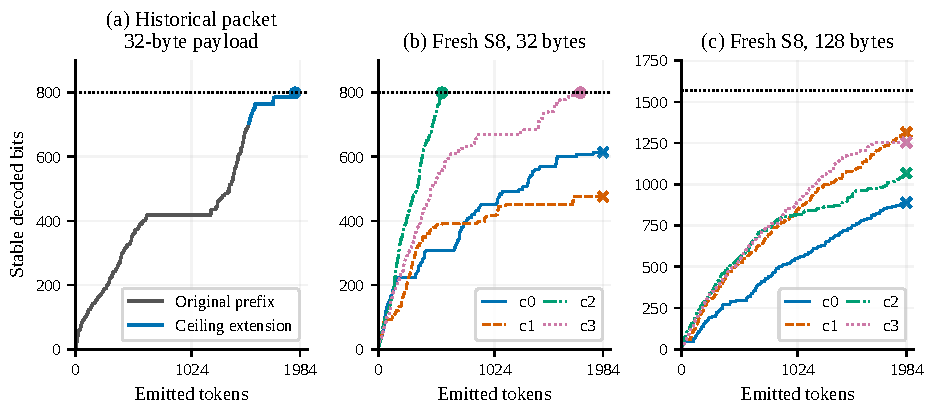
\includegraphics[width=\textwidth]{figures/figure2_capacity.pdf}
\caption{Stable decoded bits are the leading packet bits that the public interval has already fixed unambiguously. Dotted lines mark the packet target, 800 bits in (a,b) and 1,568 in (c). Panel (a) repeats one historical encrypted 32-byte packet, preserving its 1,536-token prefix and completing at 1,942 after the ceiling extension. It is diagnostic, not a new transmission. Panels (b) and (c) show every fresh S8 arithmetic trajectory, with circles for recovery and crosses for capacity exhaustion. A long text need not resolve enough bits. Each curve supplies nested checkpoints, not independent samples.}
\label{fig:capacity}
\end{figure*}

The ceiling extension preserves all four historical prefixes, including token IDs, candidate-order hashes, frequencies and interval states. The old encrypted 32-byte packet completes at 1,942 tokens and passes an independent receiver with its original authenticated binding. Both historical 196-byte packets remain incomplete at 1,984. These repeated diagnostics do not repair or replace the original 1,536-token failures.

Figure~\ref{fig:capacity} also shows the fresh S8 trajectories. R32 completes in zero of four cases by 512 tokens, one by 1,024, still one by 1,536 and two by 1,984. R128 completes in zero of four at every checkpoint. F finishes before 512 tokens at both sizes. A trajectory's later completion can support earlier-budget statements only at checkpoints after its actual stop. Partial bit progress is never authenticated recovery. All sampled steps found the required 16 candidates, so these failures are packet-capacity exhaustion, not candidate-set exhaustion.

\subsection{An Illustrative Encrypted Transmission}
\noindent The first predetermined S9 replay source uses the public context about a copper bell. Its payload is 32 synthetic binary bytes, not an English sentence. The 100-byte HPKE envelope becomes an 862-token, 3,909-byte carrier. The opening excerpt below preserves its exact characters, including the leading space. It is generated text, not a factual description of a museum object.
\begin{quote}
\VerbatimInput[fontsize=\small,breaklines=true,breaksymbolleft={},breaksymbolright={}]{generated/example_success.txt}
\end{quote}
The remainder is omitted outside the quoted excerpt. Reception uses the complete saved text, never this abbreviation. This illustrative case was selected because it is the earliest predetermined replay source, not because its wording is representative or especially natural.

From the full carrier, a public observer reconstructs 800 stable bits and the same candidate envelope. It confirms canonical replay and the necessary encapsulation representation. None of those operations reveals the 32 payload bytes or verifies their authentication tag. The intended receiver uses its private key, the exact bound profile and the recovered envelope to open HPKE, then validates the inner length. The recovered payload hash matches the original binary payload. A fresh process repeats this result. This is one transmission and one replay, not two independent successes.

\subsection{Stopping and Packet Conformance}
\noindent The S9 prospective denominators are in Table~\ref{tab:predicates}. Every B-fixed control delivers its assigned canonical text, but none reaches the 800-bit target. B-stop completes and delivers three of six attempts, at 1,186, 1,052 and 1,044 tokens. The other three exhaust 1,984 tokens internally. All six paired controls agree over their common token prefix, candidate ordering, frequencies and arithmetic state. Figure~\ref{fig:stopping} shows how changing the boundary alters which predicate is available.

\begin{table}[t]
\caption{Prospective stopping study (S9). Each check cell is pass/fail/unavailable among scorable delivered texts. Aborted attempts are listed separately and receive no wire verdict. Full format includes completion, exact end, filler and replay, but never authentication.}
\label{tab:predicates}
\centering\small
\begin{tabular}{lrrr}
\hline
Outcome & R & B-fixed & B-stop\\
\hline
Attempts & 6 & 6 & 6\\
Delivered & 4 & 6 & 3\\
Scorable & 4 & 6 & 3\\
Capacity aborts & 2 & 0 & 3\\
\hline
Valid UTF-8 & 4/0/0 & 6/0/0 & 3/0/0\\
Canonical bytes & 4/0/0 & 6/0/0 & 3/0/0\\
Support membership & 4/0/0 & 6/0/0 & 3/0/0\\
Packet target & 4/0/0 & 0/6/0 & 3/0/0\\
Exact first end & 4/0/0 & 0/0/6 & 3/0/0\\
Local filler & 4/0/0 & 0/0/6 & 1/2/0\\
Canonical replay & 4/0/0 & 0/0/6 & 0/3/0\\
KEM representation & 4/0/0 & 0/0/6 & 1/2/0\\
Full format & 4/0/0 & 0/6/0 & 0/3/0\\
\hline
\end{tabular}
\end{table}


The test requiring completion and an exact first-completion boundary accepts zero of six delivered B-fixed texts and all three delivered B-stop texts. This change is expected by construction. The complete format, which also requires filler and canonical replay, accepts zero of six B-fixed and zero of three delivered B-stop texts. All four delivered R carriers pass. Matching stopping therefore does not weaken full-format recognition in this prospective sample. It removes one reason for rejection and exposes a separate finite-packet constraint.

\begin{figure*}[t]
\centering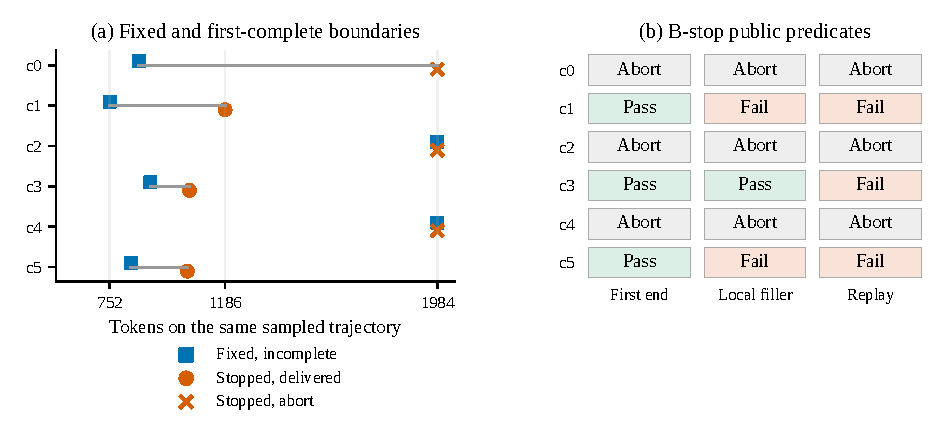
\includegraphics[width=\textwidth]{figures/figure3_stopping.pdf}
\caption{Prospective paired stopping study, one R/B-fixed/B-stop group in each of six contexts. Fixed and stopped controls share the same sampling trajectory up to their common prefix. Squares mark delivered fixed controls, all incomplete as packets. Circles mark delivered first-completion controls and crosses mark internal aborts. Reaching and ending at the target does not imply canonical replay. All three delivered stopped controls fail replay; unavailable checks on aborted outputs are not negative wire observations.}
\label{fig:stopping}
\end{figure*}

The three completed controls release 803, 801 and 814 stable bits. Local filler consistency passes only the middle case, and necessary KEM representation passes only the first. Canonical replay fails all three, first diverging at positions 1,182, 1,052 and 1,020. These overlapping checks are not independent classifiers. KEM adds no observed rejection once replay has already rejected every delivered stopped control. No authentication test is run on controls.

Retrospective S8 controls show why zero prospective format positives cannot be treated as a guarantee. Of eight R-associated fixed controls, six are incomplete and two first complete before their original ends. Reconstructing their saved public tables finds completion at 1,752 and 938 tokens. Two actual-text observer jobs then verify literal byte prefixes obtained by public tokenization. The 1,752-token prefix fails local filler and replay. The 938-token prefix passes the full format and KEM predicate. That accepted sampled prefix is a format false positive, not a fresh encrypted transmission or an independent prospective control. The original messages remain trailing-token rejections.

\subsection{An Illustrative Completed Control}
\noindent The stopped control in the stone-bench context is useful because it passes the local filler check while failing canonical replay. Its exact opening excerpt is below. Again, the remainder is omitted outside the quote, and the observer uses the complete text.
\begin{quote}
\VerbatimInput[fontsize=\small,breaklines=true,breaksymbolleft={},breaksymbolright={}]{generated/example_control.txt}
\end{quote}
This sampled control contains no encrypted payload. At token 1,052, its public arithmetic interval has fixed 801 bits. The first 800 form a candidate 100-byte packet, and the one excess bit agrees with the prescribed first filler bit. B-stop consequently delivers the message because it has reached the target, not because a packet check approved it.

Replaying the candidate packet under the encoder's deterministic midpoint convention selects a different symbol at token 1,052. The message is therefore not a canonical output of that encoder for those candidate bytes. Enough bits have become readable, yet the finite-packet convention is not satisfied. Its representation check also fails, but neither rejection requires a private key. This is one deliberately selected teaching case, not another experiment or a representative user message.

\subsection{Recognition Depends on the Generator}
\noindent Figure~\ref{fig:scores} retains individual complete-message scores and separates cohorts. In S6, F's full format accepts all 16 weighted-admissible B controls and all 16 uniform-admissible C controls, but no ordinary A control. Syntax alone therefore has no discrimination against B or C. Its KEM predicate accepts all 16 B controls but only nine of 16 C controls. Against C, format plus KEM has descriptive AUC 0.719 on 16 delivered matched pairs, with higher acceptance fixed as carrier-like. Its saved paired-cluster interval is [0.594, 0.844]. This concerns the chosen model generator and representation, not ciphertext authentication.

S6's prespecified body-score analysis excludes the initial 64 F tokens, corresponding to the 32-byte encapsulation, and applies the same exclusion to controls. Higher body surprisal yields AUC 1.0 against A and B, but 0.410 against C, each on 16 matched delivered pairs. The below-chance orientation is retained. Its C interval is [0.179, 0.609], not evidence of concealment, particularly in the presence of the representation predicate. This positional body analysis is specific to rank mapping. We never apply its fixed boundary to arithmetic output.

\begin{figure*}[t]
\centering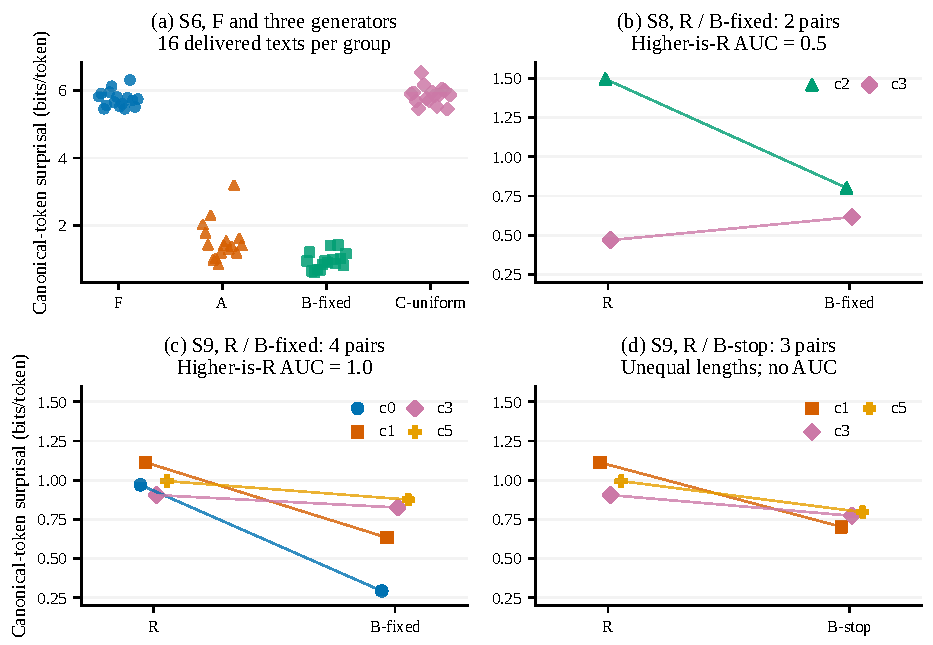
\includegraphics[width=\textwidth]{figures/figure4_scores.pdf}
\caption{Individual complete-message canonical-token surprisal scores from separate cohorts. Panel (a) contrasts F with ordinary (A), probability-weighted (B-fixed) and uniform-admissible (C) generators in S6, 16 texts per group. Panels (b) and (c) show delivered R/B-fixed pairs only, with higher score fixed as carrier-like and AUC 0.5 for two S8 pairs versus 1.0 for four S9 pairs. Colored lines keep context pairs together. Panel (d) has only three delivered R/B-stop pairs and reports no AUC; their lengths also differ. Cohorts are not pooled, and line endpoints or tokens are not independent samples.}
\label{fig:scores}
\end{figure*}

Under the common support in S8, F's complete-message surprisal AUC is 1.0 against its eight delivered matched B controls. R's AUC is 0.5 against two delivered matched B controls, both in the 32-byte class. Its descriptive interval spans [0, 1]. One context orders the R score above its control and the other orders it below. All eight R-associated controls remain available in outcome counts, but only the two paired with delivered R messages enter this score comparison. This is weak, delivery-conditioned evidence, not a demonstrated arithmetic concealment advantage.

In S9, higher-is-R complete-message surprisal gives AUC 1.0 against B-fixed on four delivered pairs. The empirical interval [1, 1] collapses because these few scores separate. It does not establish perfect population detection. Token-count AUC is mechanically 0.5 under matching, while byte-count AUC is 0.625 on the same four pairs. We retain the contrary S8 result rather than merging the two cohorts into a larger headline AUC.

Only three R/B-stop pairs are delivered. Their R scores are 1.1131, 0.9052 and 0.9943 bits/token, versus stopped-control scores 0.7027, 0.7730 and 0.7962. The encrypted carriers are also shorter in each pair. These raw differences cannot establish a length-independent score effect. No AUC or operational false-positive rate is estimated from them. Small differences between unrounded sampling probabilities and arithmetic integer tables are retained as another limitation. In S9, the largest measured per-step total-variation difference is 0.00023834. A small local difference does not imply equal distributions over complete messages.

\subsection{Computational Consequences}
\noindent The complete job costs in Table~\ref{tab:recovery} include useful work that reaches no wire output. In S8, the two successful arithmetic encrypted jobs cost 86.4 and 356.7 seconds. Their public scoring passes alone cost 24.2 and 115.4 seconds, comparable to private reconstruction. Failed 128-byte jobs average 151.0 seconds including startup, without a reception or scoring pass. Thus an abort can reduce measured job time while delivering no payload. Successful-only latency would obscure that outcome.

For S9, mean complete job time is 141.6 seconds for R, 157.4 for B-fixed and 137.9 for B-stop. Mean public scoring time, conditional on an actual delivered pass, is 39.7, 71.5 and 56.6 seconds respectively. The smaller whole-job B-stop mean does not mean cheaper successful reception, because half its attempts abort before observer scoring. The two independent receivers cost 56.0 and 58.1 seconds including startup. Canonical packet replay reuses public integer tables, but obtaining those tables requires a full model-scoring pass. Public observability has a measurable computational cost.

\section{DISCUSSION AND LIMITATIONS}
\label{sec:discussion}
\noindent The experiments support separating three questions. Can a finite packet accumulate enough information before the context limit? Does the emitted UTF-8 reconstruct correctly? Which public constraints distinguish complete delivered messages from a named cover generator? These questions have different failure denominators and different computational costs. Treating any one as a proxy for the others would misread the retained evidence.\aidraft

S8 format separation did not isolate midpoint consistency: its controls were incomplete or trailed past first completion. S9 matches stopping without conditioning on replay or KEM. All three delivered controls then satisfy the boundary but fail replay. The accepted historical prefix shows that such failure is not inevitable. This separates mechanisms without estimating their population frequencies.

S6 prevents a universal public-inversion claim. Expected-length extraction is common under its constrained generators. Representation helps against one generator and adds nothing against another, while scores can overlap or reverse. Permitted observer information and cover distributions are part of the claim. Uniform-admissible controls are a diagnostic reference, not human communication.

The experiments use one quantized model/backend and selected short contexts. The final six share a template and confound context, key and payload. Capacity selects recognition samples. Only two fresh R messages deliver in S8 and four in S9. Controls, tokens, repeated observers and replays do not enlarge those genuine-carrier counts. Prospective freezing within each exploratory cohort does not make it a final held-out test.

Our support, midpoint extension and endpoint are specific conventions. Other arithmetic termination rules may differ. The 128-byte failures are bounded negative results, not a general impossibility, and successful examples would not prove distributional security. No validated keyed comparator is evaluated under its actual shared-secret assumptions.

Confidentiality relies on HPKE, not a low recognition score. The study supplies no chosen-covertext theorem, length hiding, recipient anonymity or post-compromise protection. Authentication gates payload delivery but does not identify the sender. These unchanged-text studies establish no robustness to edits, paraphrase or normalization. Application replay protection is separate from independent reception checks.

The ingredients are established. The defensible addition is retained actual-text evidence linking finite-packet progress, an unchanged-prefix extension, paired stopping controls and separate conformance predicates. It shows concretely why recovery, a token sampler and a format verdict cannot substitute for a complete-message evaluation. It does not establish a generally superior transport.

\section{CONCLUSION}
\label{sec:conclusion}
\noindent Our bounded studies retain exact rank-profile recovery, arithmetic capacity aborts and generator-dependent recognition. Independent reconstruction identifies low-information trajectories; one ceiling extension enables some smaller packets while all four fresh larger packets still fail. Matching first completion removes boundary rejection on delivered controls but leaves replay rejection in all three. A separate historical accepted prefix prevents interpreting this as universal detection. Finite-packet delivery, stopping and conformance require separate evaluation from actual UTF-8, with explicit abort conditioning.\aidraft

\section*{AI-USE DISCLOSURE}
\label{sec:disclosure}
\noindent OpenAI Codex assisted the abstract and Sections 1 through 7 with source checking, drafting and revision, and assisted the scripts and layout for all figures and tables \cite{openai2026codex}. The session identifies the GPT-6 model family; an exact serving-build identifier is unavailable. Figures 2 through 4 and numerical tables are generated from retained experimental records, not invented or image-generated data. Figure 1 is a scripted explanatory schematic. No new model inference or experimental case was run to prepare this draft. The human authors remain responsible for technical accuracy, attribution and the final submission. This non-identifying disclosure is included outside acknowledgments for anonymous review.

\bibliographystyle{apalike}
\bibliography{references}
\end{document}
